\documentclass[10pt,a4paper]{article}
\usepackage[UTF8,fontset = windows]{ctex}
\setCJKmainfont[BoldFont=黑体,ItalicFont=楷体]{华文中宋}
\usepackage{amssymb,amsmath,amsfonts,amsthm,mathrsfs,dsfont,graphicx}
\usepackage{ifthen,indentfirst,enumerate,color,titletoc}
\usepackage{tikz}
\usetikzlibrary{arrows,calc}
\usepackage[bf,small,indentafter,pagestyles]{titlesec}
\usepackage[top=1in, bottom=1in,left=0.8in,right=0.8in]{geometry}
\renewcommand{\baselinestretch}{1.65}
\newtheorem{defi}{定义~}
\newtheorem{eg}{例~}
\newtheorem{ex}{~}
\newtheorem{rem}{注~}
\newtheorem{thm}{定理~}
\newtheorem{coro}{推论~}
\newtheorem{axiom}{公理~}
\newtheorem{prop}{性质~}

\newcommand{\blank}[1]{\underline{\hbox to #1pt{}}}
\newcommand{\bracket}[1]{(\hbox to #1pt{})}

\begin{document}

\begin{center}
    赋能正确率小于$0.75$的题目
\end{center}

{\tiny 1,10,0.512}  若双曲线的一条渐近线为$x+2y=0$, 且双曲线与抛物线$y=x^2$的准线仅有一个公共点, 则此双曲线的标准方程为\blank{50}.

%赋能2


{\tiny 2,7,0.488} 若函数$f(x)=\begin{cases}    2^x, & x\le 0, \\ -x^2+m, & x>0 \end{cases}$的值域为$(-\infty ,1]$, 则实数$m$的取值范围是\blank{50}.

{\tiny 3,10,0.605} 有以下命题:\\
\textcircled{1} 若函数$f(x)$既是奇函数又是偶函数, 则$f(x)$的值域为$\{0\}$; \\
\textcircled{2} 若函数$f(x)$是偶函数, 则$f(|x|)=f(x)$;\\
\textcircled{3} 若函数$f(x)$在其定义域内不是单调函数, 则$f(x)$不存在反函数;\\
\textcircled{4} 若函数$f(x)$存在反函数${{f}^{-1}}(x)$, 且${{f}^{-1}}(x)$与$f(x)$不完全相同, 则$f(x)$与${{f}^{-1}}(x)$图像的公共点必在直线$y=x$上; \\
其中真命题的序号是\blank{50}(写出所有真命题的序号).

% 赋能4


{\tiny 4,4,0.523} 若$(1+x)^5=a_0+a_1x+a_2x^2+\cdots+a_5x^5$, 则$a_1+a_2+\cdots+a_5=$\blank{50}.

{\tiny 4,5,0.750} 设$k\in \mathbf{R}$, $\dfrac{y^2}{k}-\dfrac{x^2}{k-2}=1$表示焦点在$y$轴上的双曲线, 则半焦距的取值范围是\blank{50}.

{\tiny 4,8,0.727} 已知圆$C:x^2+y^2+2kx+2y+k^2=0$($k\in \mathbf{R}$)和定点$P(1,-1)$, 若过$P$可以作两条直线与圆$C$相切, 则$k$的取值范围是\blank{50}.

{\tiny 4,9,0.750} 如图, 在直三棱柱$ABC-A_1B_1C_1$中, $\angle ABC=90^\circ$, $AB=BC=1$, 若$A_1C$与平面$B_1BCC_1$所成的角为$\dfrac{\pi}{6}$, 则三棱锥$A_1-ABC$的体积为\blank{50}.
\begin{center}
    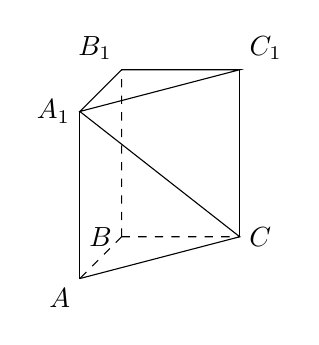
\begin{tikzpicture}[scale = 1.5]
        \draw [dashed] (0,0) -- (1,0) node [right] {$C$} coordinate (C) (0,0) -- (225:0.5) node [below left] {$A$} coordinate (A) (0,0) node [left] {$B$} coordinate (B) -- (0,{sqrt(2)}) node [above left] {$B_1$} coordinate (B1);
        \draw (A) --+ (0,{sqrt(2)}) node [left] {$A_1$} coordinate (A1);
        \draw (C) --+ (0,{sqrt(2)}) node [above right] {$C_1$} coordinate (C1);
        \draw (A1) -- (B1) -- (C1) -- (A1) -- (C) -- (A);
    \end{tikzpicture}
\end{center}

{\tiny 8,8,0.705} 已知数列$\{a_n\}$的通项公式为$a_n=n^2+bn$, 若数列$\{a_n\}$是单调递增数列, 则实数$b$的取值范围是\blank{50}.

{\tiny 13,10,0.545} 若$a_n$是$(2+x)^n$($n\in \mathbf{N}^*$, $n\ge 2$, $x\in \mathbf{R}$)展开式中$x^2$项的二项式系数, 则$\displaystyle\lim_{n\to\infty}(\dfrac 1{a_2}+\dfrac 1{a_3}+\cdots+\dfrac1{a_n})=$\blank{50}.

% 赋能14


{\tiny 14,9,0.674} 已知抛物线$C$的顶点为坐标原点, 双曲线$\dfrac{x^2}{25}-\dfrac{y^2}{144}=1$的右焦点是$C$的焦点$F$. 若斜率为$-1$, 且过$F$的直线与$C$交于$A,B$两点, 则$|AB|=$\blank{50}.

{\tiny 14,10,0.744} 直角坐标系$xOy$内有点$P(-2,-1)$, $Q(0,-2)$, 将$\triangle POQ$绕$x$轴旋转一周, 则所得几何体的体积为\blank{50}.

% 赋能15


{\tiny 18,6,0.595} 过点$P(-2,1)$作圆$x^2+y^2=5$的切线, 则该切线的点法向式方程是\blank{50}.

{\tiny 18,9,0.619} 已知$\triangle ABC$的三个内角$A,B,C$所对边长分别为$a,b,c$, 记$\triangle ABC$的面积为$S$, 若$S=a^2-(b-c)^2$, 则内角$A=$\blank{50}(结果用反三角函数值表示).

{\tiny 18,10,0.381} 已知函数$f(x)=\left|\dfrac1{|x|-1}\right|$, 关于$x$的方程$f^2(x)+bf(x)+c=0$有$7$个不同实数根, 则实数$b,c$满足的关系式是\blank{50}.
% 赋能19


{\tiny 19,8,0.721} 已知点$A(2,3)$、点$B(-2,\sqrt3)$, 直线$l$过点$P(-1,0)$, 若直线$l$与线段$AB$相交, 则直线$l$的倾斜角的取值范围是\blank{50}.

{\tiny 19,10,0.581} 向量$\overrightarrow{i}$、$\overrightarrow{j}$是平面直角坐标系$x$轴、$y$轴的基本单位向量, 且$|\overrightarrow a-\overrightarrow i|+|\overrightarrow a-2\overrightarrow j|=\sqrt5$, 则$|\overrightarrow a+2 \overrightarrow i|$的取值范围为\blank{50}.

% 赋能20


{\tiny 21,10,0.750} 如图, 向量$\overrightarrow{OA}$与$\overrightarrow{OB}$的夹角为$120^\circ$, $|\overrightarrow{OA}|=2$, $|\overrightarrow{OB}|=1$, $P$是以$O$为圆心、$|\overrightarrow{OB}|$为半径的弧$\overset\frown{BC}$上的动点, 若$\overrightarrow{OP}=\lambda \overrightarrow{OA}+\mu \overrightarrow{OB}$, 则$\lambda \mu$的最大值是\blank{50}.
\begin{center}
    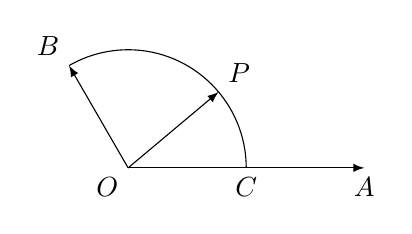
\begin{tikzpicture}[scale = 1.5, >=latex]
        \draw [->] (0,0) node [below left] {$O$} -- (2,0) node [below] {$A$};
        \draw [->] (0,0) --+ (120:1) node [above left] {$B$};
        \draw [->] (0,0) --+ (40:1) node [above right] {$P$};
        \draw (1,0) node [below] {$C$} arc (0:120:1);
    \end{tikzpicture}
\end{center}

% 赋能22


{\tiny 23,10,0.568} 已知函数$f(x)=x|2x-a|-1$有三个零点, 则实数$a$的取值范围为\blank{50}.

% 赋能24


{\tiny 24,9,0.682} 同时掷两枚质地均匀的骰子, 则两个点数之积不小于$4$的概率为\blank{50}.

{\tiny 25,10,0.605} 若不等式$(-1)^n\cdot a<3+\dfrac{(-1)^{n+1}}{n+1}$对任意正整数$n$恒成立, 则实数$a$的取值范围是\blank{50}.

%赋能26


{\tiny 26,10,0.535} 已知函数$f(x)=\cos x(\sin x+\sqrt3\cos x)-\dfrac{\sqrt3}2$, $x\in \mathbf{R}$. 设$\alpha>0$, 若函数$g(x)=f(x+\alpha)$为 奇函数, 则$\alpha$的值为\blank{50}.

%赋能27


{\tiny 30,5,0.698} 若$(x+2)^n=x^n+ax^{n-1}+\cdots+bx+c \ (n\in \mathbf{N}^*, \ n\ge 3)$, 且$b=4c$, 则$a$的值为\blank{50}.

{\tiny 30,6,0.558} 某空间几何体的三视图如图所示, 则该几何体的侧面积是\blank{50}.
\begin{center}
    \begin{tikzpicture}[>=latex]
        \draw (0,0) circle (1);
        \draw (-1,-1.1) -- (-1,-1.3) (1,-1.1) -- (1,-1.3);
        \draw [->] (-0.2,-1.2) -- (-1,-1.2);
        \draw [->] (0.2,-1.2) -- (1,-1.2);
        \draw (0,-1.2) node {$4$};
        \draw (0,-1.6) node {俯视图};
        \draw (-1,2) -- (1,2) -- (0,5) -- cycle;
        \draw (0,1.4) node {主视图};
        \draw (-1,1.9) -- (-1,1.7) (1,1.9) -- (1,1.7);
        \draw [->] (-0.2,1.8) -- (-1,1.8);
        \draw [->] (0.2,1.8) -- (1,1.8);
        \draw (0,1.8) node {$4$};
        \draw (1.1,2) -- (1.3,2) (1.1,5) -- (1.3,5);
        \draw [->] (1.2,3.2) -- (1.2,2);
        \draw [->] (1.2,3.8) -- (1.2,5);
        \draw (1.2,3.5) node {$6$};
        \draw (2,2) -- (4,2) -- (3,5) -- cycle;
        \draw (3,1.4) node {左视图};
        \draw (2,1.9) -- (2,1.7) (4,1.9) -- (4,1.7);
        \draw [->] (2.8,1.8) -- (2,1.8);
        \draw [->] (3.2,1.8) -- (4,1.8);
        \draw (3,1.8) node {$4$};
        \draw (4.1,2) -- (4.3,2) (4.1,5) -- (4.3,5);
        \draw [->] (4.2,3.2) -- (4.2,2);
        \draw [->] (4.2,3.8) -- (4.2,5);
        \draw (4.2,3.5) node {$6$};
    \end{tikzpicture}
\end{center}

{\tiny 30,10,0.744} 已知椭圆$x^2+\dfrac{y^2}{b^2}=1\ (0<b<1)$, 其左、右焦点分别为$F_1$, $F_2$, $|F_1F_2|=2c$. 若此椭圆上存在点$P$, 使$P$到直线$x=\dfrac1c$的距离是$|PF_1|$与$|PF_2|$的等差中项, 则$b$的最大值为\blank{50}.

% 赋能31


{\tiny 31,10,0.721} 甲与其四位朋友各有一辆私家车, 甲的车牌尾数是$0$, 其四位朋友的车牌尾数分别是$0$, $2$, $1$, $5$, 为遵守当地4月1日至5日$5$天的限行规定(奇数日车牌尾数为奇数的车通行, 偶数日车牌尾数为偶数的车通行), 五人商议拼车出行, 每天任选一辆符合规定的车, 但甲的车最多只能用一天, 则不同的用车方案总数为\blank{50}.

% 赋能32


{\tiny 33,9,0.524} 若从正八边形的$8$个顶点中随机选取$3$个顶点, 则以它们作为顶点的三角形是直角三角形的概率是\blank{50}.

{\tiny 34,7,0.558} 各项均不为零的数列$\{a_n\}$的前$n$项和为$S_n$.  对任意$n\in \mathbf{N}^*$, $\overrightarrow{m_n}=(a_{n+1}-a_n,2a_{n+1})$
都是直线$y=kx$的法向量. 若$\displaystyle\lim_{n\to\infty}S_n$存在, 则实数$k$的取值范围是\blank{50}.

{\tiny 38,9,0.721} 小明和小红各自掷一颗均匀的正方体骰子, 两人相互独立地进行. 则小明掷出的点数不大于$2$或小红掷出的点数不小于$3$的概率为\blank{50}.

{\tiny 39,10,0.512} 设奇函数$f(x)$的定义域为$\mathbf{R}$, 当$x>0$时,$f(x)=x+\dfrac{m^2}x-1$(这里$m$为正常数). 若$f(x)\le m-2$对一切$x\le 0$成立, 则$m$的取值范围为\blank{50}.

% 赋能40


{\tiny 40,10,0.721} 已知$x,y\in \mathbf{R}$, 且满足$\begin{cases} \sqrt3x+y\le 4 \sqrt3, \\  \sqrt3x-y\ge 0,\\ y\ge 0. \end{cases}$ 若存在$\theta \in \mathbf{R}$使得$x\cos \theta +y\sin \theta +1=0$成立, 则点$P(x,y)$构成的区域面积为\blank{50}.

% 赋能41


{\tiny 43,1,0.744} 已知$A=(-\infty,a]$, $B=[1,2]$, 且$A\cap B\ne \varnothing$, 则实数$a$的范围是\blank{50}.

{\tiny 43,4,0.674} 长方体的对角线与过同一个顶点的三个表面所成的角分别为$\alpha$, $\beta$, $\gamma$, 则$\cos^2\alpha+\cos^2\beta+\cos^2\gamma =$\blank{50}.

{\tiny 45,10,0.581} 平面上三条直线$x-2y+1=0$, $x-1=0$, $x+ky=0$, 如果这三条直线将平面划分为六个部分, 则实数$k$的取值组成的集合$A=$\blank{50}.

% 赋能46


{\tiny 47,10,0.744} 若函数$f(x)={\log_a}(x^2-ax+1)\ (a>0, \ a\ne 1)$没有最小值, 则$a$的取值范围是\blank{50}.

% 赋能48


{\tiny 49,10,0.605} 设变量$x,y$满足条件$\begin{cases}  x-y\ge 0, \\ 2x+y\le 2, \\ y\ge 0, \\ x+y\le m, \end{cases}$ 若该条件表示的平面区域是三角形, 则实数$m$的取值范围是\blank{50}.

% 赋能50


{\tiny 50,4,0.721} 已知两个不同向量$\overrightarrow{OA}=(1,m)$, $\overrightarrow{OB}=(m-1,2)$, 若$\overrightarrow{OA}\perp\overrightarrow{AB}$, 则实数$m=$\blank{50}.

{\tiny 53,9,0.395} 已知四面体$ABCD$中, $AB=CD=2$, $E$, $F$分别为$BC$, $AD$的中点, 且异面直线$AB$与$CD$所成的角为$\dfrac{\pi}3$, 则$EF$=\blank{50}.

{\tiny 54,9,0.558} 曲线$\begin{cases} x=1-\dfrac{\sqrt5}5 t, \\ y=-1+\dfrac{2\sqrt5}5t, \end{cases}$($t$为参数)与曲线$\begin{cases} x=\sin \theta \cdot \cos \theta, \\ y=\sin \theta +\cos \theta,  \end{cases}$($\theta$为参数)的公共点的坐标为\blank{50}.





\end{document}